%fitts law in use (methods)
\section{Performance Test} \label{sec:M:fittsLaw}

%present how the fitts gui works
%subject reaches target
%variables for the performance metrics are recorded 
%performance metrics are calculated (but are first presented in results)

As stated in \secref{sec:BG:validatingPerformance} the theory behind Fitts Law, this project will utilize a modified Fitts' Law task consisting of a virtual target reaching test to evaluate the progress of subjects going through user training. The proposed modified Fitts' law test utilizes the performance metrics of, throughput, path efficiency, overshoot, stopping distance and completion rate. The following section describes how the Fitts' Law task has been implemented in this project.

\subsection{Virtual target reaching test} \label{sub:M:targetReachingTest}

The virtual targets reaching test was implemented into the same GUI used for data acquisition and user training, first mentioned in \secref{sec:M:dataAcquisition}. 
%Different functions have been build into the GUI to enable switching between different usages by the press of a button.
When enabling the target reaching test in the GUI the subject was met with the interface shown in \figref{fig:fittsLawTask}. Here the subjects controlled the position of the cursor by performing movements shown above, below, and on the sides of the borders of the grid area. Thus, extension of the hand would move the cursor to the right of the grid, and flexion would move the cursor to the left. Similarly, radial and ulnar deviation moved the cursor up and down respectively. This approach was used to improve the intuitiveness of the control where the direction of the cursor relate to the directions subjects will perform hand movements.
%, when placed as instructed in the protocol, \appref{sec:protocol:experiment} \fxnote{appref virker måske bedre en en secref til protokollen når vi får bygget en ordentlig main med et rigtigt appedix så protokollerne heller ikke står under bibliografien}
Subjects controlled the size of the cursors red area by opening and closing the hand, where an open hand increases the area and a closed hand decreases the area. \\
Each target was presented by an area with a center and an outer circle. Targets existed in three sizes in order to test opened and closed hand degree of freedom. The target reaching test consisted of reaching a total of 16 targets which each appeared for 15 seconds at positions around the center of the grid area. The order of appearance was fixed but different for each trial but the same across subjects, thus individual subjects will experience the targets as appearing in a new order with each trial. 

\begin{figure}[H] 
	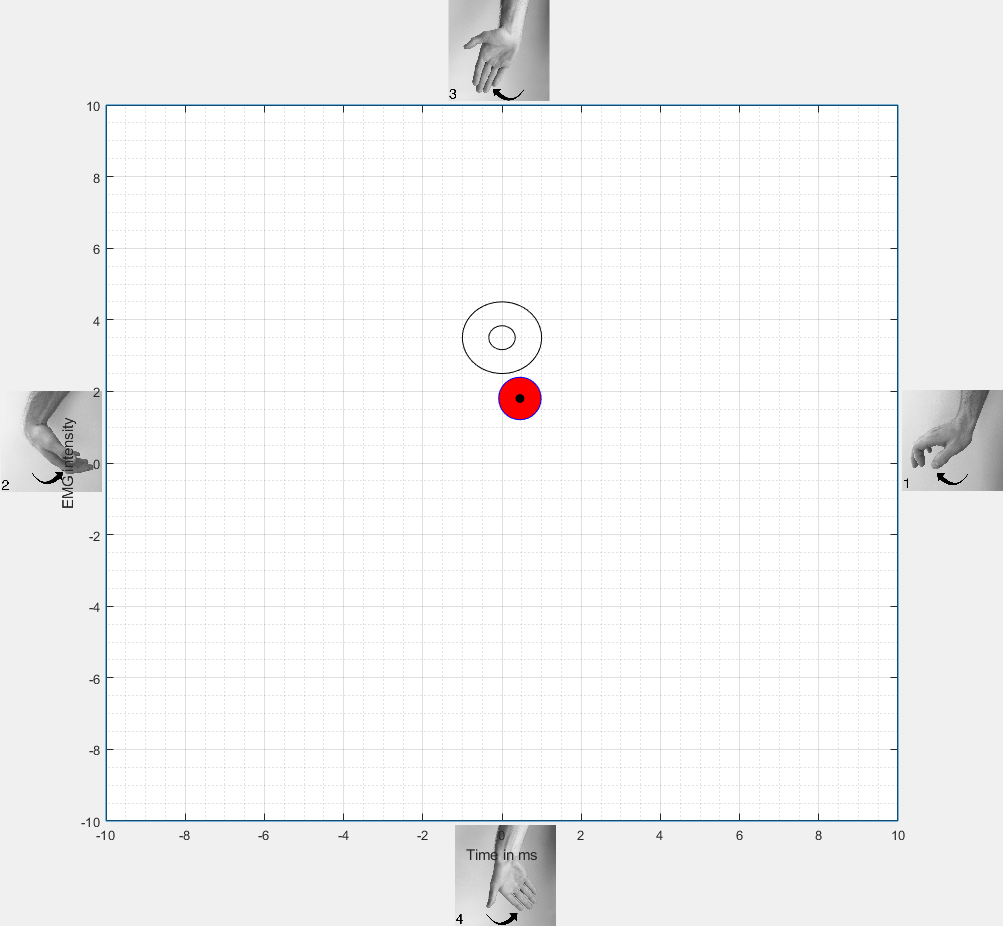
\includegraphics[width=0.7\textwidth]{figures/xBackground/perftestGUI}
	\caption{The implemented interface for the modified Fitts' Law task. The grid was the area in which the subject must reach targets with the controlled cursor. The cursor  the red circle area with the black dot in the center. Targets were shown as a circle area with an bigger outer circle. Performing the shown movement would move the cursor in the direction of the picture.}
	\label{fig:fittsLawTask}
\end{figure}

Subjects had to reach the targets inner circle with the cursor dot and expand or decrease the red area of the cursor to reach a size close to that of the target. A moderate size threshold had been implemented to make it possible to reach targets, without a 100\% accuracy of control. If a subject reached a target, the cursor would change color from red to green, and thus the subject withholds this position for a 1 second dwell the cursor changed to blue, and a bell chime will sound to indicate that the target was reached. The cursor position was reset to the center of the grid area and the color of the cursor would revert back to red. If a target was not reached within 15 seconds the current target would disappear, a new target would be shown and the cursor position would be set to the center of the grid area. The approach of resetting the cursor position after each target is to equalize the path for every subject. 

As mentioned earlier multiple performance metrics was recorded during the target reaching test. One of these measures were throughput which depend on the index of difficulty for the targets, as stated in \secref{sub:BG:fitts}. The ID was calculated for all targets in the 3-dimensional target space shown on INDSÆT FIGUR. 


The configuration of targets in the test resulted in 8 combinations of width and distance. The smaller circle has the same width in each target thereby possessing the same area in which the cursor center has to be within. The index of difficulty for the targets used in the modified Fitts' law test can be seen in \tabref{tab:M:ID}

\begin{table}[H]
	\centering
	\caption{The index of difficulty used in the modified Fitts' law test.}
	\label{tab:M:ID}
	\begin{tabular}{l|l|l}
		
		Distance & Width         & Index of Difficulty \\ \hline
		28.0     & $\frac{1}{3}$ & 6.41                \\ \hline
		24.5     & $\frac{1}{3}$ & 6.22                \\ \hline
		22.0     & $\frac{1}{3}$ & 6.01                \\ \hline
		18.5     & $\frac{1}{3}$ & 5.82                \\ \hline
		16.0     & $\frac{1}{3}$ & 5.61                \\ \hline
		13.0     & $\frac{1}{3}$ & 5.32                \\ \hline
		12.5     & $\frac{1}{3}$ & 5.27                \\ \hline
		9.5      & $\frac{1}{3}$ & 4.88                \\ \hline
	\end{tabular}
\end{table}



A trace of the cursor movement throughout the whole test is recorded to decide the subjects path deviation from the optimal path to calculate the path efficiency and distances to targets. An example of a cursor trace is shown in \figref{fig:cursorTrace}. 

\begin{figure}[H] 
	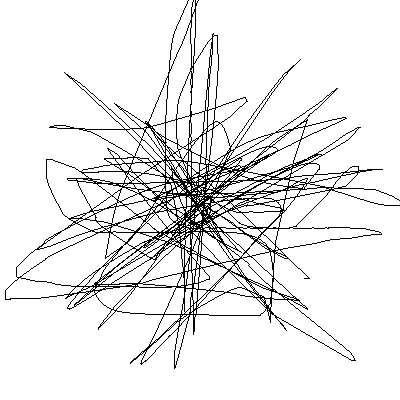
\includegraphics[width=1\textwidth]{figures/pMethods/cursorTrace}
	\caption{The trace of the cursor movement after a target reaching test. This information is not visible or shown to subjects.}
	\label{fig:cursorTrace}
\end{figure}

The number of times a target is reached and exited without completing the dwell time, is recorded and used to calculate subjects overshoot. Similarly to tracking the travelled distance of the cursor inside the grid area, the travelled distance inside of each target is also recorded to calculate the stopping distance. The number or reached targets is recorded. The total amount of time possible to use in completing the target reaching test is: $16 ~targets~*~15s = 240s = 4~min$. 

Following the completion of recording target reaching test data from all subjects the performance metrics introduced in \secref{sub:BG:fitts} are calculated and presented in the Results: \chapref{chap:Results}.




